\documentclass{beamer}
\usetheme{Boadilla}
% \usepackage{beamerthemesplit} // Activate for custom appearance


\setbeamertemplate{navigation symbols}{}
\setbeamertemplate{footline}{}

\addtobeamertemplate{navigation symbols}{}{%
    \usebeamerfont{footline}%
    \usebeamercolor[fg]{footline}%
    \hspace{1em}%
    \insertframenumber/\inserttotalframenumber
}

\usepackage{gensymb}
\usepackage[absolute,overlay]{textpos}
\usepackage{braket}
\usepackage{bm}

\title{Tunable Testbed for Detection and Attribution}
\subtitle{IDAG Workshop 2018}

\author[shortname]{Nathan Lenssen \inst{1} \and Dorit Hammerling \inst{2} \and Alexis Hannart \inst{3}}
\date{March 14, 2018}

\institute[shortinst]{\inst{1} Columbia University, Lamont-Doherty Earth Observatory \and %
                      \inst{2} National Center for Atmospheric Resarch \inst{3} Ouranos}
                      

\titlegraphic{\vspace*{1.5cm} 
\includegraphics[height=1cm]{Images/ldeoLogo.png}\hspace*{4.75cm}~%
   
\includegraphics[height=1cm]{Images/nsfLogo.jpg}
}

\newcommand{\Prob}{\ensuremath{\mathbb{P}}}
\newcommand{\E}{\ensuremath{\mathbb{E}}}
\newcommand{\V}{\ensuremath{\text{Var}}}
\newcommand{\C}{\ensuremath{\text{Cov}}}
\newcommand{\insitu}{\emph{in situ }}
\newcommand{\iid}{\ensuremath{\stackrel{\text{iid}}{\sim}}}

\newcommand{\light}[1]{\textcolor{gray}{#1}}

\setbeamerfont{framesource}{size=\tiny}

\newcommand{\source}[1]{\begin{textblock*}{4cm}(0.1 cm,8.9cm)
    \begin{beamercolorbox}[ht=0.5cm,left]{framesource}
        \usebeamerfont{framesource}\usebeamercolor[fg]{framesource} Source: {#1}
    \end{beamercolorbox}
\end{textblock*}}

% shortcut for bold
\def\*#1{\bm{#1}}
\def\C{\textbf{\text{C}}}
\def\W{\textbf{\text{W}}}

\begin{document}

\frame{\titlepage}


\begin{frame}
\frametitle{SAMSI Working Group/Collaborators}
\begin{itemize}
\item The Statistical and Applied Mathematical Sciences Institute (SAMSI) Is conducting a year-long research program on Mathematical and Statistical Methods for Climate and the Earth System (CLIM)
\item My research is as a member of the CLIM working group on Detection and Attribution led by Dorit Hammerling 
\item The testbed is joint with Alexis Hannart and a continuation of \cite{hannart16}



\end{itemize}
 
 \vfill    
\hfill     
\includegraphics[width=1.5in]{Images/samsilogo.jpg} %merra anomaly field 
\end{frame}

% give a sense of why the problem is so complex
% list of high-level goals from the testbed
\begin{frame}
\frametitle{Testbed Motivation}
A flexible and tunable testbed will allow researchers working on detection and attribution methods to:
\begin{itemize}
\item Evaluate methods by comparing estimated and true parameter values
\begin{itemize}
\item Performance scaling as a function of sample size/dimensionality
\end{itemize}
\item Simulate real-world scenarios to enable testbed results to represent applications
\begin{itemize}
\item Tunable variety of climate response patterns and climate variability covariances
\end{itemize}
\item Determine robustness of methods through perturbations of testbed parameters
\item \structure{Compare multiple D+A methods on variety of scenarios}

\end{itemize}

\end{frame}


\begin{frame}
\frametitle{Roadmap of Presentation}

\begin{itemize}
\item[(I)] Generative Statistical Model for Detection and Attribution
\begin{itemize}
\item Ordinary Least Squares
\item Error-in-Variable Formulation
\item Sources of Variability
\end{itemize}
\item[(II)] Major Testbed Components 
\begin{itemize}
\item Observed vs. Latent Data/Parameters
\item Simulation of Forced Responses
\item Covariances of Climate and Observational Variability
\end{itemize}
\item[(III)] Results and Applications
\end{itemize}
\end{frame}


%%%%%%%%%%%%%%%%%%%%%%%%
% (I) Introduce formulation used in presentation
%%%%%%%%%%%%%%%%%%%%%%%%

%%%
% (A) EIV formulation
%%%

% OLS
\begin{frame}
\frametitle{Classical Formulation of Detection and Attribution}
\framesubtitle{Ordinary Least Squares (OLS)}

\structure{Observed Quantities:}
\begin{itemize}
\item[$\*y$:] The \alert{observed} climate response of interest 
\item[$\*X^*$] The \alert{model-simulated} forcing responses $\*X^* = (\*x^*_1, \dots, \*x^*_m , \dots, \*x^*_M)$
\end{itemize}

\pause

\begin{block}{}
\vspace*{-5pt}\setlength\belowdisplayshortskip{0pt}
\begin{equation*}
\*y = \*X^* \*\beta + \* u
\end{equation*}
\end{block}

\pause
\structure{Statistical Parameter of Interest:}
\begin{itemize}
\item[$\*\beta$] Estimation of $\beta >0$ provides detection, inference (CIs) gives us attribution
\end{itemize}

\structure{Climate Variability:}
\begin{itemize}
\item[$\*u$] The error due to climate variability where $\*u \sim \mathcal{N}(0, \C)$
\item[$\C$] Estimated through model control runs
\end{itemize}
\end{frame}

% EIV model 1: Introduction
\begin{frame}
\frametitle{Statistical Formulation of Detection and Attribution}
\framesubtitle{Error-in-Variable (EIV)}
\structure{Observed Quantities:}
\begin{itemize}
\item[$\*y$] The climate response of interest 
\item[$\*X$] The \alert{noisy} responses to forcings $\*X = (\*x_1, \dots, \*x_m , \dots, \*x_M)$
\end{itemize}

\pause

\begin{block}{}
\vspace*{-\baselineskip}\setlength\belowdisplayshortskip{0pt}
\begin{align*}
\*y &= \*X^* \*\beta + \*u_y \nonumber \\
\*X &= \*X^* + \*U \:
\end{align*}
\end{block}

\pause

\structure{Latent Quantities:}
\begin{itemize}
\item[$\*y^*$] The idealized climate response where $\*y^* = \*X^* \*\beta$
\item[$\*X^*$] The idealized responses to forcings $\*X^* = (\*x_1^*, \dots, \*x_M^*)$
\end{itemize}

\structure{Climate Variability:}
\begin{itemize}
\item[$\*u_y$] As OLS formulation with $\*u_y \sim \mathcal N(0, \C)$
\item[$\*U$] The error on the forcing responses due to climate variability
\setlength\abovedisplayskip{0pt}
\setlength\belowdisplayskip{0pt}
\[
\*U = (\*u_1, \dots, \*u_M) \stackrel{\text{iid}}{\sim} \mathcal{N}(0,\C)
\]

\end{itemize}

\end{frame}

% EIV model 2: Multimodel ensembles
%\begin{frame}
%\frametitle{Statistical Formulation of Detection and Attribution}
%\framesubtitle{Error-in-Variable (EIV): Multimember Ensembles}
%
%For a given forcing $m$, we run ensemble of size $L_m$
%\[
%\*x_m = ( \*x_m^{(1)}, \dots \*x_m^{(\ell)}, \dots, \*x_m^{(L_m)}) \, , \qquad  \*x_m^{(\ell)} \iid \mathcal{N}(\*x^*_m, \C)
%\]
%
%The \structure{ensemble mean} of the $m^{\text{th}}$ forced response is 
%\begin{align*}
%\overline{\*x_m} &= \frac{1}{L_m} \sum_{\ell=1}^{L_m} \*x_m^{(\ell)} \, , \qquad  \overline{\*x_m} \sim \mathcal{N}\left(\*x^*_m, L_m^{-1}\,\C\right)
%\end{align*}
%
%Rewriting in the error-in-variable formulation
%\[
%\overline{\*x_m} = \*x^*_m +L_m^{-1/2} \*u_m
%\]
%Or for all forcing responses with $\*L = \text{diag}(L_1, \dots, L_M)$
%\begin{exampleblock}{}
%\vspace*{-5pt}\setlength\belowdisplayshortskip{0pt}
%\[
%\overline{\*X} = \*X^* +\*L^{-1/2} \*U
%\]
%\end{exampleblock}
%\end{frame}


% EIV Model 3: Incoporation of multimodel ensembles
%\begin{frame}
%\frametitle{Statistical Formulation of Detection and Attribution}
%\framesubtitle{Error-in-Variable (EIV): Multimember Ensembles}
%
%\begin{exampleblock}{}
%\vspace*{-5pt}\setlength\belowdisplayshortskip{0pt}
%\[
%\overline{\*X} = \*X^* +\*L^{-1/2} \*U
%\]
%\end{exampleblock}
%
%Plugging into our full error in variable formulation:
%
%\begin{block}{}
%\vspace*{-\baselineskip}\setlength\belowdisplayshortskip{0pt}
%\begin{alignat*}{3}
%\*y &= \*X^* \*\beta + \*u_y \nonumber  \qquad  &\*u_y &\sim \mathcal N(0,\C) \\
%\overline{\*X} &= \*X^* + \*L^{-1/2} \*U \qquad    &\*u_m &\iid \mathcal N(0,\C)  \:
%\end{alignat*}
%\end{block}
%
%\begin{itemize}
%\item[$\overline{\*X}$] The ensemble means $\overline{\*X} = (\overline{\*x_1}, \dots, \overline{\*x_M})$ 
%\item[$\*L$] The ensemble sizes $\*L = (L_1, \dots, L_M)$
%\item[$\*U$] The forcing variability matrix $\*U = (\*u_1, \dots, \*u_M)$
%\end{itemize}
%\end{frame}

%%%
% (A) obs formulation
%%%

% true, realize, observed responses
\begin{frame}
\frametitle{Statistical Formulation of Detection and Attribution}
\framesubtitle{Observed Response Variability}

The \alert{incomplete} expression for the climate response $\*y$ is
\begin{alertblock}{}
\vspace*{-5pt}\setlength\belowdisplayshortskip{0pt}
\begin{equation*}
\*y = \*X^* \*\beta + \* u_y  \, , \qquad \*u_y \sim \mathcal{N} (0,\C) 
\end{equation*}	
\end{alertblock}

We propose three different $\*y$ states to fully incorporate all of the sources of variability.

\begin{itemize}
\item[$\*y^*$] The \structure{idealized} climate response (latent) \hfill $\*y^* = \*X^* \*\beta \qquad \qquad \qquad$
\item[$\*y_{rel}$] The \structure{realized} climate response (latent) \hfill $\*y_{rel} = \*y^* + \*u_Y \,\; \qquad \qquad$
\item[$\*y_{obs}$] The \structure{observed} climate response \hfill $\*y_{obs} = \*y_{rel} + \*\varepsilon_Y \, \qquad \qquad$
\begin{itemize}
\item With observational error $\* \varepsilon_Y \sim \mathcal N(0,\W)$
\end{itemize}
\end{itemize}

\begin{exampleblock}{}
\vspace*{-\baselineskip}\setlength\belowdisplayshortskip{0pt}
\begin{alignat*}{3}
\*y_{rel} &= \*X^* \*\beta + \*u_y \nonumber  \qquad  &\*u_y &\sim \mathcal N(0,\C) \\
\*y_{obs} &= \*y_{rel} + \*\varepsilon_y &\*\varepsilon_y &\sim \mathcal N(0,\W)
\end{alignat*}
\end{exampleblock}

\end{frame}


%% ensembles of distribution 
%\begin{frame}
%\frametitle{Statistical Formulation of Detection and Attribution}
%\framesubtitle{Observed Response Variability}
%
%\begin{block}{}
%\vspace*{-\baselineskip}\setlength\belowdisplayshortskip{0pt}
%\begin{alignat*}{3}
%\*y_{rel} &= \*X^* \*\beta + \*u_y \nonumber  \qquad  &\*u_y &\sim \mathcal N(0,\C) \\
%\*y_{obs} &= \*y_{rel} + \*\varepsilon_y &\*\varepsilon_y &\sim \mathcal N(0,\W)
%\end{alignat*}
%\end{block}
%
%\structure{Total Observation Variability:} Since the observational and climate variability errors are independent, condense in terms of $\*\nu = \*u_y + \*\varepsilon_y$
%\begin{align*}
%\*y_{obs} &= \*y_{rel} + \*\varepsilon_y \\
%&= \*X^* \* \beta + \*\nu \: , \qquad \* \nu \sim \mathcal{N}(0,\C + \W)
%\end{align*}
%
%\begin{itemize}
%\item [] \alert{Note:} Flexibility to add additional variability terms to $\*\nu$
%\begin{itemize}
%\item Linear approximation error (from statistical model)
%\item Climate model error
%\end{itemize}
%\end{itemize}
%\end{frame}
%
%% ensembles of observational ensemble
%\begin{frame}
%\frametitle{Statistical Formulation of Detection and Attribution}
%\framesubtitle{Observed Response Variability}
%
%\begin{block}{}
%\vspace*{-\baselineskip}\setlength\belowdisplayshortskip{0pt}
%\begin{alignat*}{3}
%\*y_{rel} &= \*X^* \*\beta + \*u_y \nonumber  \qquad  &\*u_y &\sim \mathcal N(0,\C) \\
%\*y_{obs} &= \*y_{rel} + \*\varepsilon_y &\*\varepsilon_y &\sim \mathcal N(0,\W)
%\end{alignat*}
%\end{block}
%
%\structure{Observational Ensembles:} Following the notation of the multimember ensembles with $L_y$ as the size of the observational ensemble
%\begin{align*}
%\*Y_{obs} &= ( \*y_{obs}^{(1)}, \cdots,  \*y_{obs}^{(L_y)}) \\
% &=  \*Y_{rel} + (  \*\varepsilon_y^{(1)}, \cdots,   \*\varepsilon_y^{(L_y)}) \: , \qquad \*\varepsilon_y^{(\ell)} \iid \mathcal N(0,\W) \\
%\end{align*}
%
%\alert{Information about $\W$ may be from gained from multiple observations, but information about $\C$ does not increase!}
%
%\end{frame}
%



\begin{frame}
\frametitle{Statistical Formulation of Detection and Attribution}
\framesubtitle{Full Model}

\structure{Full Error-in-Variable Model:}
\begin{block}{}
\vspace*{-\baselineskip}\setlength\belowdisplayshortskip{0pt}
\begin{alignat*}{3}
\*y_{obs} &= \*y_{rel} + \*\varepsilon_y  \qquad \quad &\*\varepsilon_y &\sim \mathcal N(0,\W)\\
\*y_{rel} &= \*X^* \*\beta + \*u_y \nonumber  \qquad  &\*u_y &\sim \mathcal N(0,\C) \\
\overline{\*X} &= \*X^* + \*L^{-1/2} \*U \qquad    &\*u_m &\iid \mathcal N(0,\C)  \:
\end{alignat*}
\end{block}

\pause

\structure{Scale-Variant Error-in-Variable Model:}
\begin{exampleblock}{}
\vspace*{-\baselineskip}\setlength\belowdisplayshortskip{0pt}
\begin{alignat*}{3}
\*y_{obs} &= \*y_{rel} + \*\varepsilon_y  \qquad \quad &\*\varepsilon_y &\sim \mathcal N(0,\W)\\
\*y_{rel} &= \*X^* \*\beta + \*u_y \nonumber  \qquad  &\*u_y &\sim \mathcal N(0,{\color{red} \alpha^{-1}}\,\C) \\
\overline{\*X} &= \*X^* + \*L^{-1/2} \*U \qquad    &\*u_m &\stackrel{\text{ind}}{\sim} \mathcal N(0,{\color{red}\gamma_m^{-1}} \, \C)  \:
\end{alignat*}
\end{exampleblock}

\alert{Dorit will talk about fitting this model!}
\end{frame}




%%%%%%%%%%%%%%%%%%%%%%%%
% (II) Introduce Testbed
%%%%%%%%%%%%%%%%%%%%%%%%

\begin{frame}
\frametitle{Roadmap of Presentation}

\begin{itemize}
\item[(I)] Generative Statistical Model for Detection and Attribution
\begin{itemize}
\item Ordinary Least Squares
\item Error-in-Variable Formulation
\item Sources of Variability
\end{itemize}
\item[(II)] \alert{Major Testbed Components}
\begin{itemize}
\item \alert{Observed vs. Latent Data/Parameters}
\item \alert{Simulation of Forced Responses}
\item \alert{Covariances of Climate and Observational Variability}
\end{itemize}
\item[(III)] Results and Applications
\end{itemize}
\end{frame}



% Observed Objects
\begin{frame}
\frametitle{Data and Parameters of Interest}

\begin{block}{}
\vspace*{-\baselineskip}\setlength\belowdisplayshortskip{0pt}
\begin{alignat*}{3}
\*y_{obs} &= \*y_{rel} + \*\varepsilon_y  \qquad \quad &\*\varepsilon_y &\sim \mathcal N(0,\W)\\
\*y_{rel} &= \*X^* \*\beta + \*u_y \nonumber  \qquad  &\*u_y &\sim \mathcal N(0,\alpha^{-1}\,\C) \\
\overline{\*X} &= \*X^* + \*L^{-1/2} \*U \qquad    &\*u_m &\stackrel{\text{ind}}{\sim} \mathcal N(0,\gamma_m^{-1} \, \C)  \:
\end{alignat*}
\end{block}

\alert{Observed Objects:}

\begin{itemize}
\item[$\*X$] Observed forcing response ensembles
\begin{align*}
\*X &= (\*x_1, \dots, \*x_M)\\
&= \left(  [\*x_1^{(1)}, \dots, \*x_1^{(L_1)} ], \dots, [\*x_M^{(1)}, \dots, \*x_M^{(L_M)} ] \right)
\end{align*}
\item[$\*Y_{obs}$] Observed climate response ensemble
\[
\*Y_{obs} = (\*y_{obs}^{(1)}, \dots, \*y_{obs}^{(L_y)})
\]
\item[$\*X_0$] Control runs from the climate model used in forcing response experiments
\[
\*X_0 = (\*X_0^{(1)}, \dots, \*X_0^{(L_0)})
\]
\end{itemize}

\end{frame}

% Observed Objects
\begin{frame}
\frametitle{Data and Parameters of Interest}

\begin{block}{}
\vspace*{-\baselineskip}\setlength\belowdisplayshortskip{0pt}
\begin{alignat*}{3}
\*y_{obs} &= \*y_{rel} + \*\varepsilon_y  \qquad \quad &\*\varepsilon_y &\sim \mathcal N(0,\W)\\
\*y_{rel} &= \*X^* \*\beta + \*u_y \nonumber  \qquad  &\*u_y &\sim \mathcal N(0,\alpha^{-1}\,\C) \\
\overline{\*X} &= \*X^* + \*L^{-1/2} \*U \qquad    &\*u_m &\stackrel{\text{ind}}{\sim} \mathcal N(0,\gamma_m^{-1} \, \C)  \:
\end{alignat*}
\end{block}


\alert{Latent Objects}

\begin{itemize}
\item[$\theta$] The statistical parameters in the model
\[
\theta = \{\beta, \alpha, \*\gamma, \C, \W\}
\]
\item[$\*X^*$] True forcing response $\,\,\*X = (\*x_1, \dots, \*x_M)$
\item[$\*y^*$] True climate response $\*y^* = \*X \* \beta$
\item[$\*y_{rel}$] Realized climate response
\end{itemize}

\end{frame}

% Simulation Outline
\begin{frame}
\frametitle{Simulation Procedure}

\begin{block}{}
\vspace*{-\baselineskip}\setlength\belowdisplayshortskip{0pt}
\begin{alignat*}{3}
\*y_{obs} &= \*y_{rel} + \*\varepsilon_y  \qquad \quad &\*\varepsilon_y &\sim \mathcal N(0,\W)\\
\*y_{rel} &= \*X^* \*\beta + \*u_y \nonumber  \qquad  &\*u_y &\sim \mathcal N(0,\alpha^{-1}\,\C) \\
\overline{\*X} &= \*X^* + \*L^{-1/2} \*U \qquad    &\*u_m &\stackrel{\text{ind}}{\sim} \mathcal N(0,\gamma_m^{-1} \, \C)  \:
\end{alignat*}
\end{block}

For a simulation of fixed dimensionality:
\begin{itemize}
\item[1)] Set/Simulate fixed objects $\theta = \{ \beta, \alpha, \*\gamma , \C, \W \}$ and $\*X^*$
\begin{itemize}
\item$\*X^*$, $\C$, and $\W$ according to simulation modules
\end{itemize}
\item[\light{2a)}] \light{Simulate the observed forcing response ensembles $\*x_m$ 
\[
\*x^{(\ell)}_m \iid \mathcal N ( \*x_m^*, \C)
\]
\item[\light{2b)}]Simulate the realized climate response $\* y_{rel}$
\[
\*y_{rel} \sim \mathcal N ( \*X^* \* \beta, \C)
\]}
\item[\light{3)}] \light{Simulate the observed climate response ensemble $\*Y_{obs}$}
\light{\[
\*y_{obs}^{(\ell)} \iid \mathcal N ( y_{rel}, \W)
\]}
\end{itemize}
\end{frame}

%% Testbed Modules
%\begin{frame}
%\frametitle{1) Simulate Fixed Objects} 
%\framesubtitle{Testbed Modules}
%\begin{itemize}
%\item[(M1)] True Forcing Response $\*X^*$
%\begin{itemize}
%\item Fixed spatial field that may be randomly generated
%\item Currently use a Mat\'ern random field
%\end{itemize}
%\item[(M2)] Climate Variability Covariance $\C$
%\begin{itemize}
%\item Use modified exponential eigenfunction (rectangular harmonics)
%\end{itemize}
%\item[(M3)] Observational Error Covariance $\W$
%\begin{itemize}
%\item Currently independent, heteroskedastic 
%\end{itemize}
%\end{itemize}
%
%\end{frame}


% X* generation

\begin{frame}
\frametitle{(M1) True Forcing Response $\*X^*$}
\framesubtitle{Simulated Mat\'ern Patterns}

\begin{columns}
\begin{column}{0.5\textwidth}
\begin{itemize}
  \item Fields simulated with covariance matrices according to the Mat\'ern covariance function
  \item Flexible statistical model that can be fit to replicate climate fields
  \begin{itemize}
  \item Simulate land-sea interface
  \end{itemize}
  \item Random generation of $\*X^*$ allows for robustness testing of methods
\end{itemize}
\end{column}
\begin{column}{0.5\textwidth}
    \begin{center}
     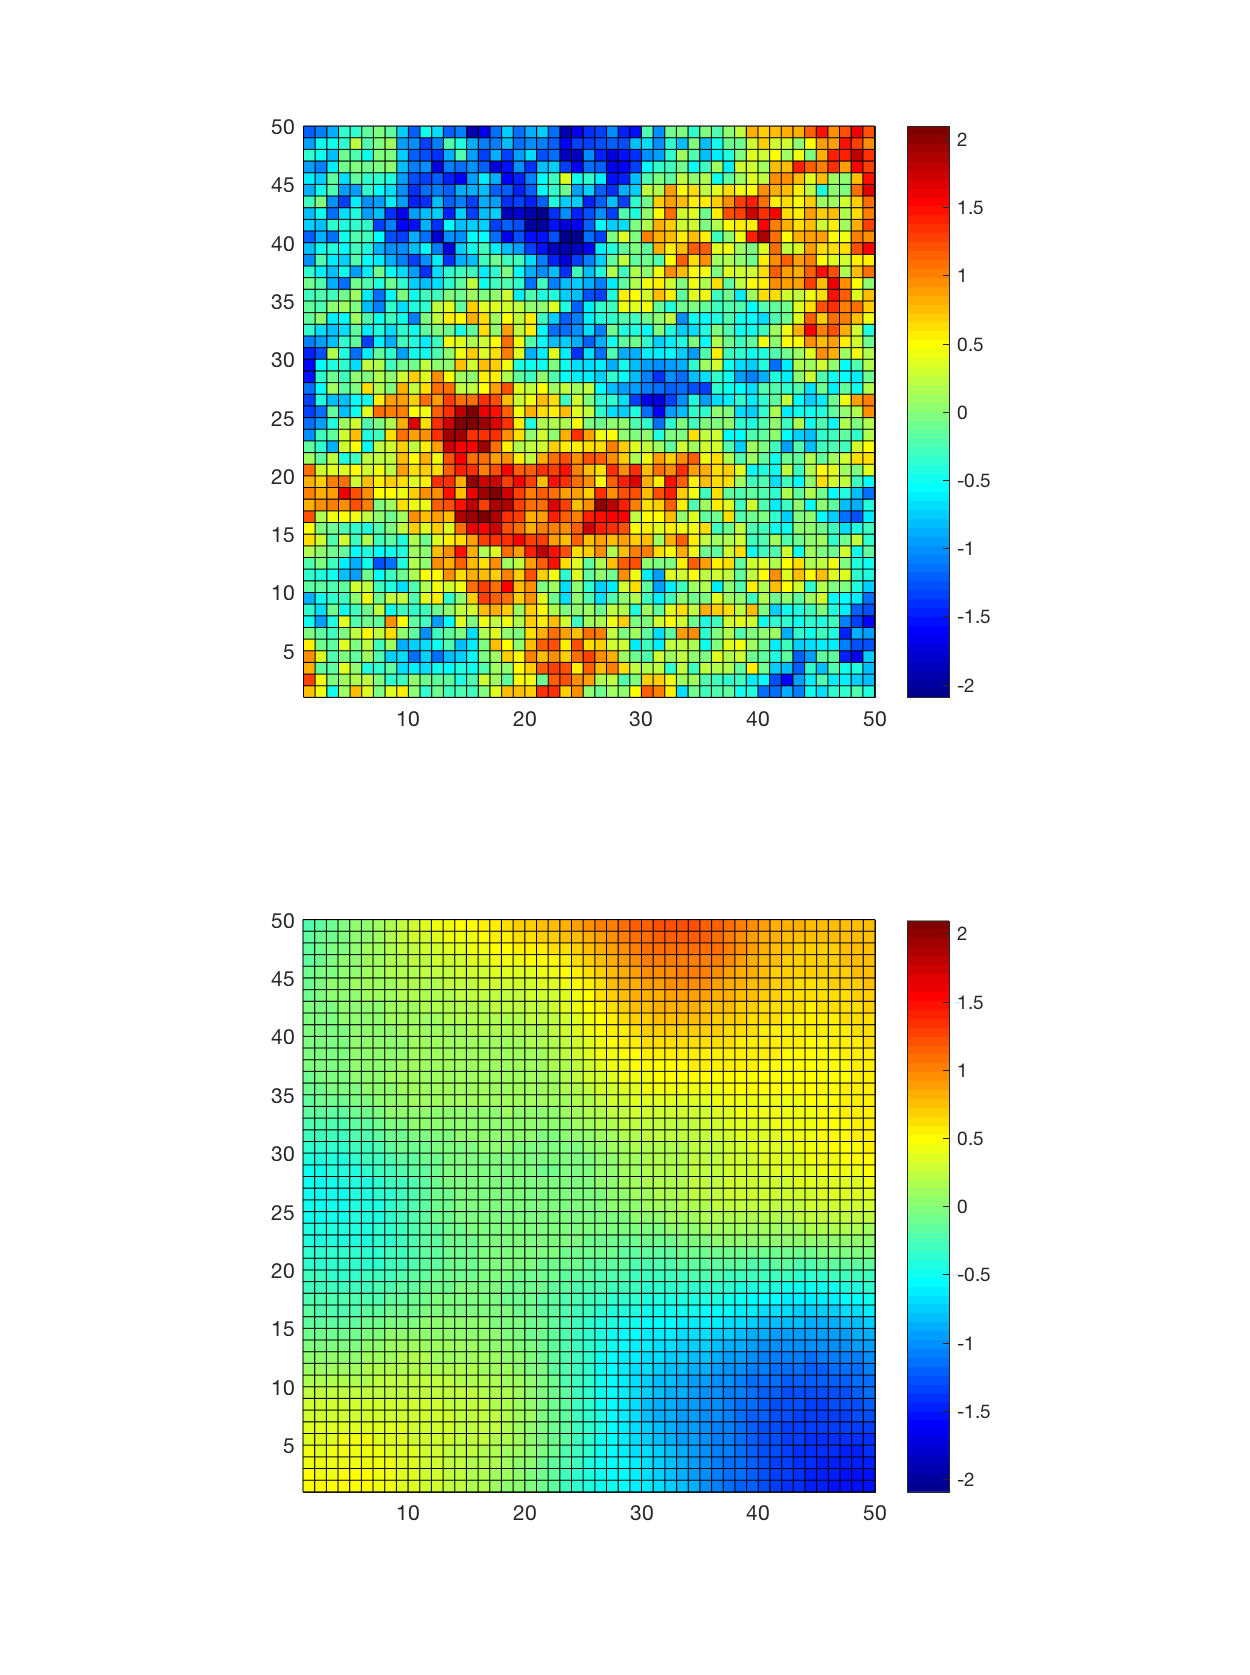
\includegraphics[width=\textwidth]{Images/maternExample.png} %merra anomaly field 
     \end{center}
\end{column}
\end{columns}

\end{frame}

\begin{frame}
\frametitle{(M1) True Forcing Response $\*X^*$}
\framesubtitle{Simulated Patterns}

\begin{columns}
\begin{column}{0.5\textwidth}
    \begin{center}
     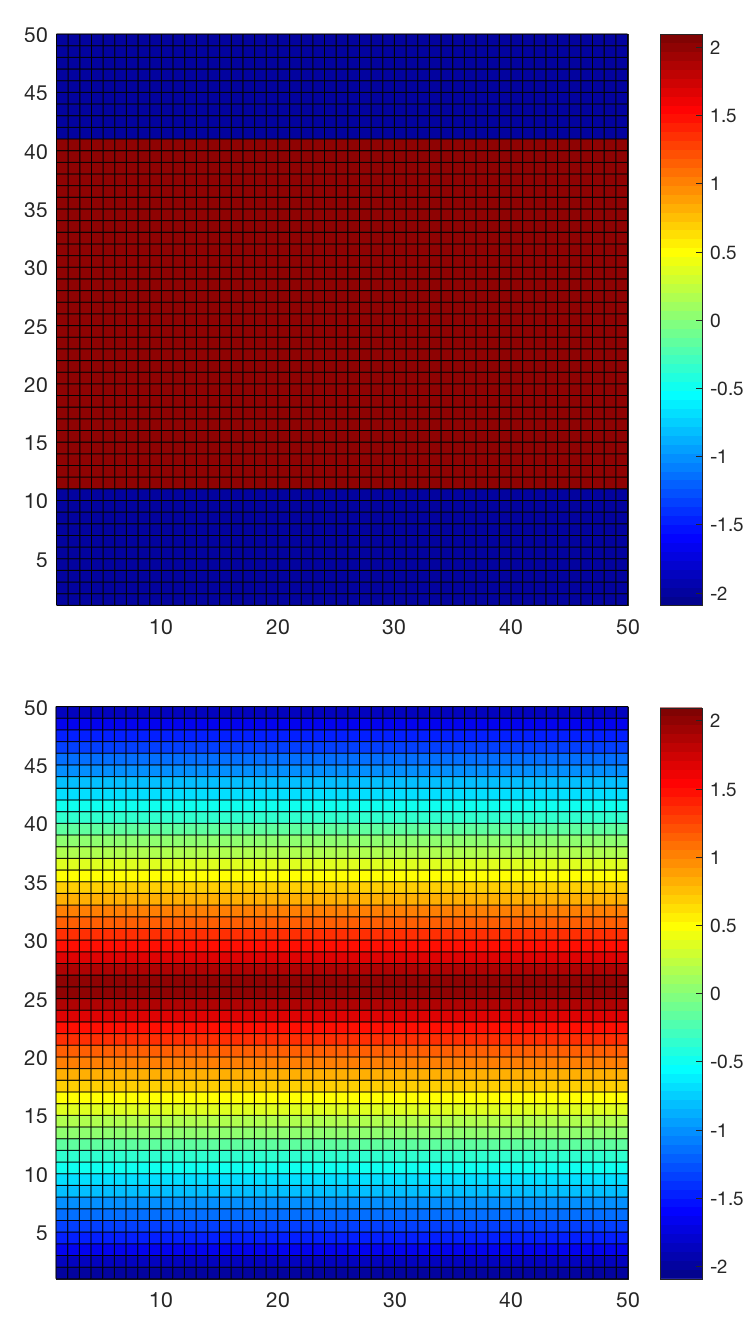
\includegraphics[width=0.75\textwidth]{Images/simpleXExample.png} %merra anomaly field 
     \end{center}
\end{column}
\begin{column}{0.5\textwidth}
    \begin{center}
     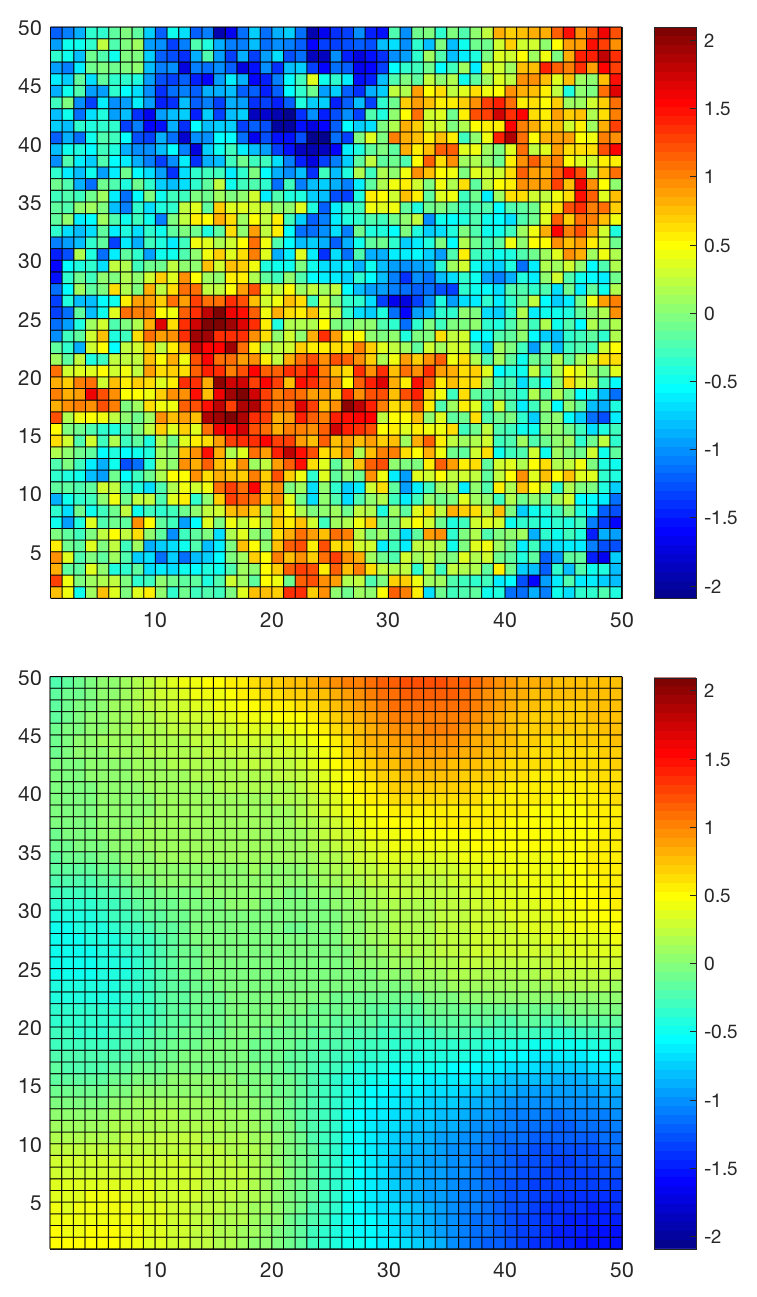
\includegraphics[width=0.75\textwidth]{Images/maternExample2.png} %merra anomaly field 
     \end{center}
\end{column}
\end{columns}

\end{frame}


% C generation

\begin{frame}
\frametitle{(M2) Climate Variability Covariance $\C$}

\begin{columns}
\begin{column}{0.5\textwidth}
\begin{itemize}
  \item Exponential covariance function too smooth and regular for climate applications like precipitation
  \item \structure{Goal:} Generate non-stationary, non-isotropic covariance matrix
  \item \alert{Issue:} Difficult to create and guarantee invertibility!
\item \structure{Solution:} Modify the eigenvalues of a decomposed exponential covariance matrix 
\end{itemize}
\end{column}
\begin{column}{0.5\textwidth}
    \begin{center}
     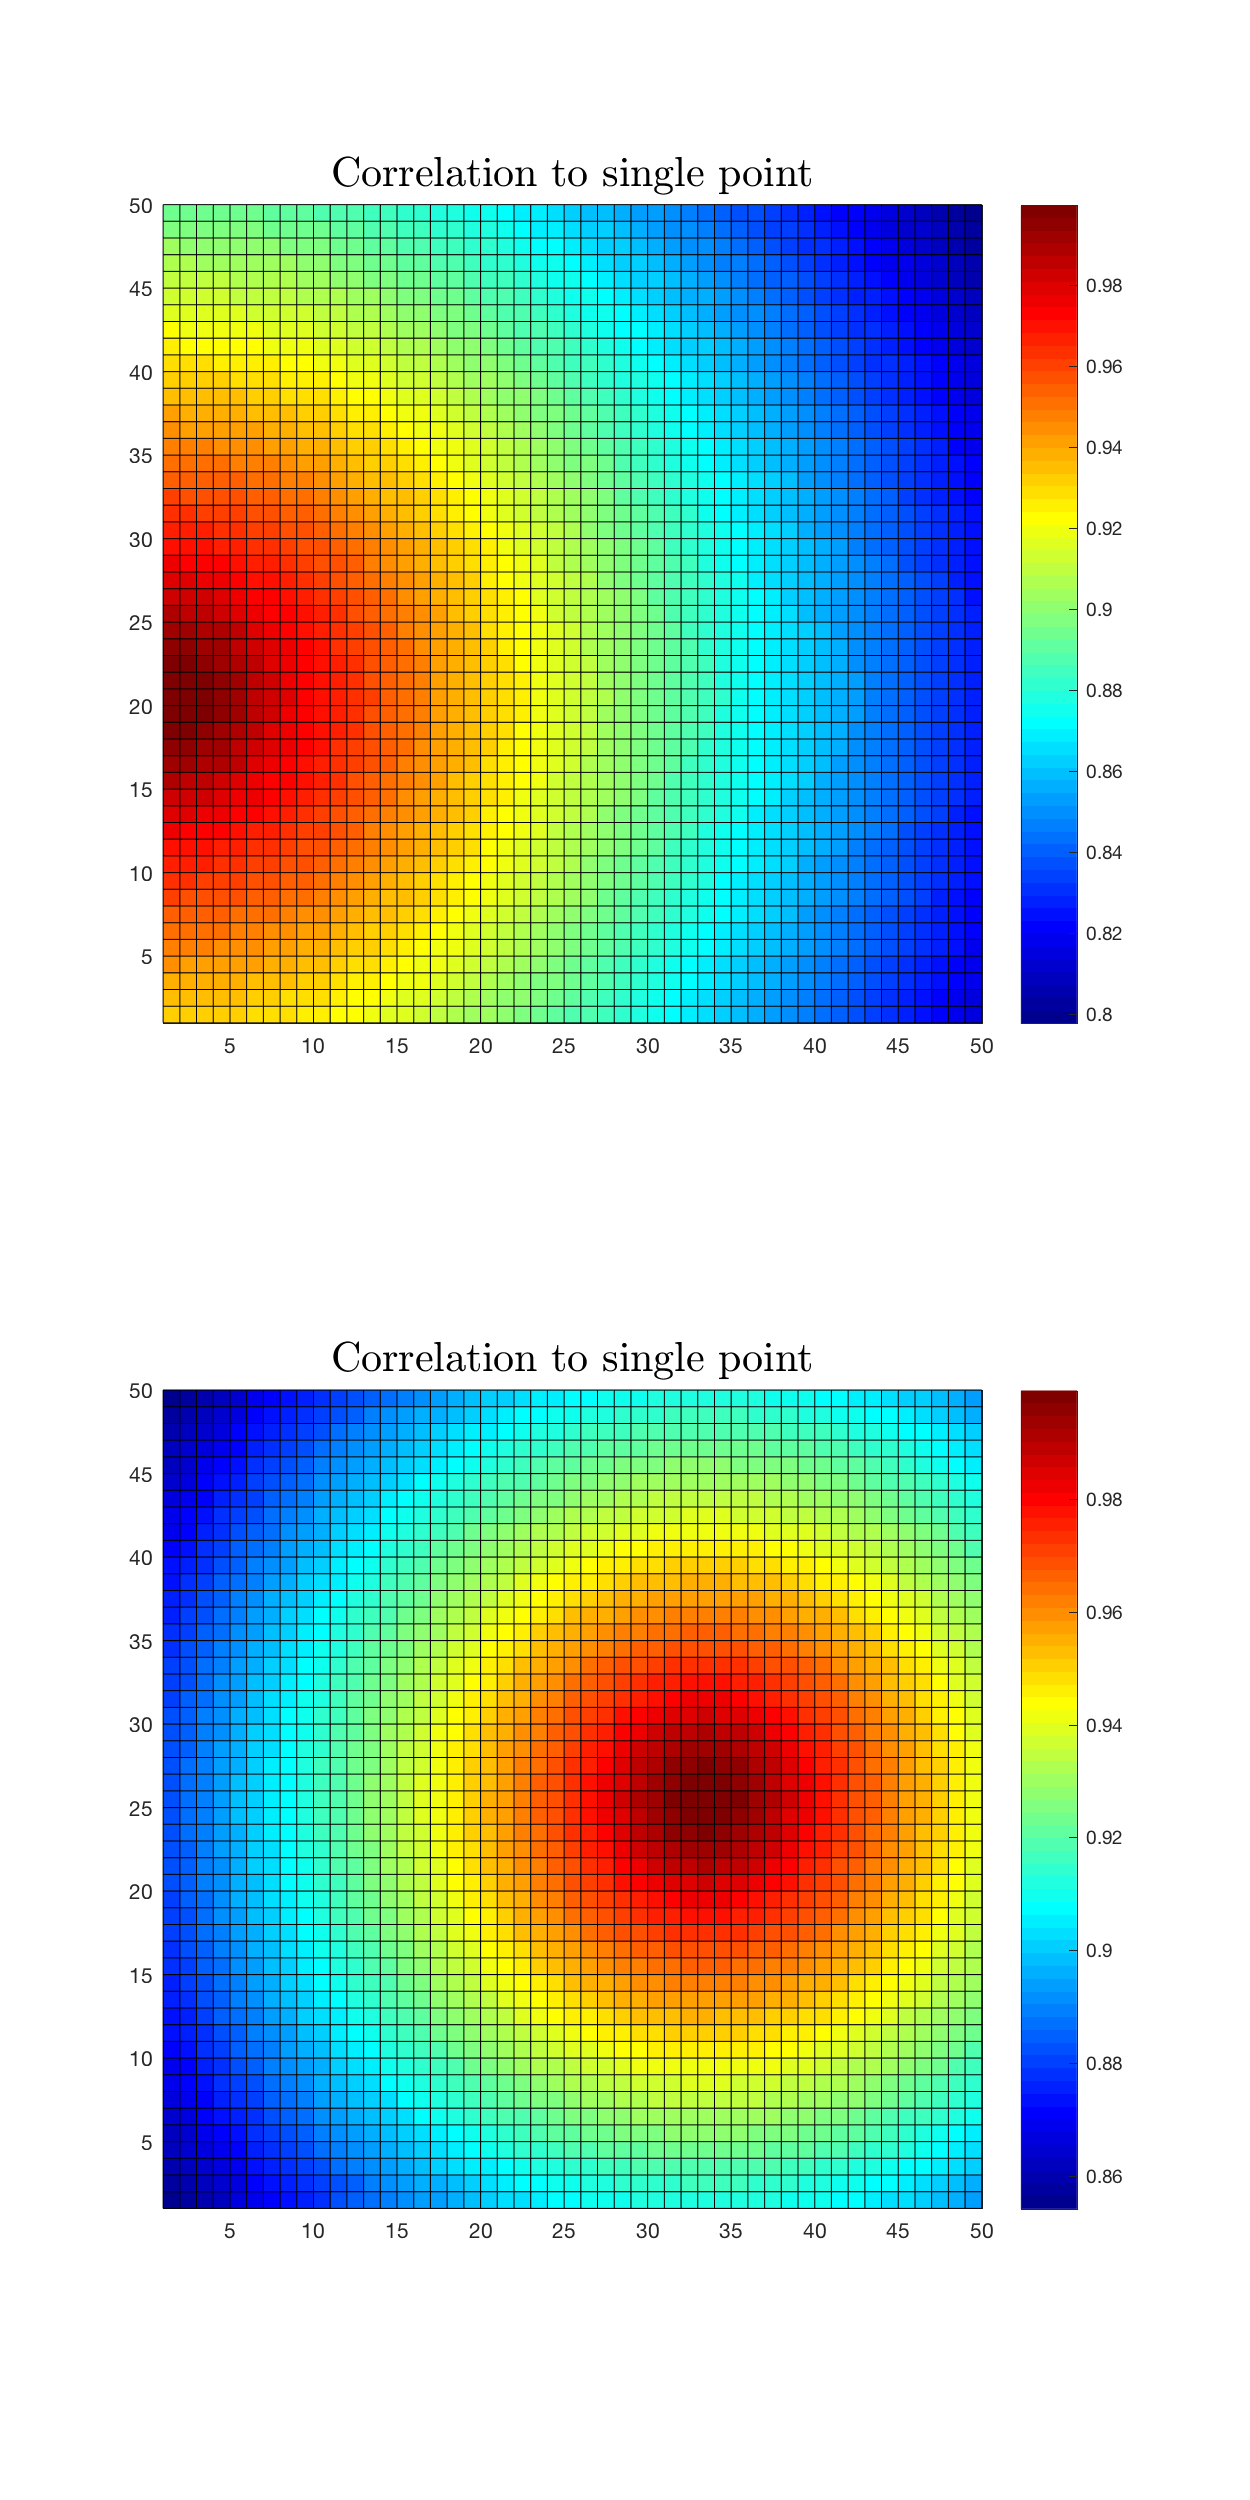
\includegraphics[width=0.7\textwidth]{Images/expoCorrelation.png} 
     \end{center}
\end{column}
\end{columns}

\end{frame}


% rec basis
\begin{frame}
\frametitle{Eigenfunctions of Exponential Covariance Function}
\framesubtitle{$\Sigma_{exp} = V_{exp} \Lambda V_{exp}^{-1}$}
\begin{center}
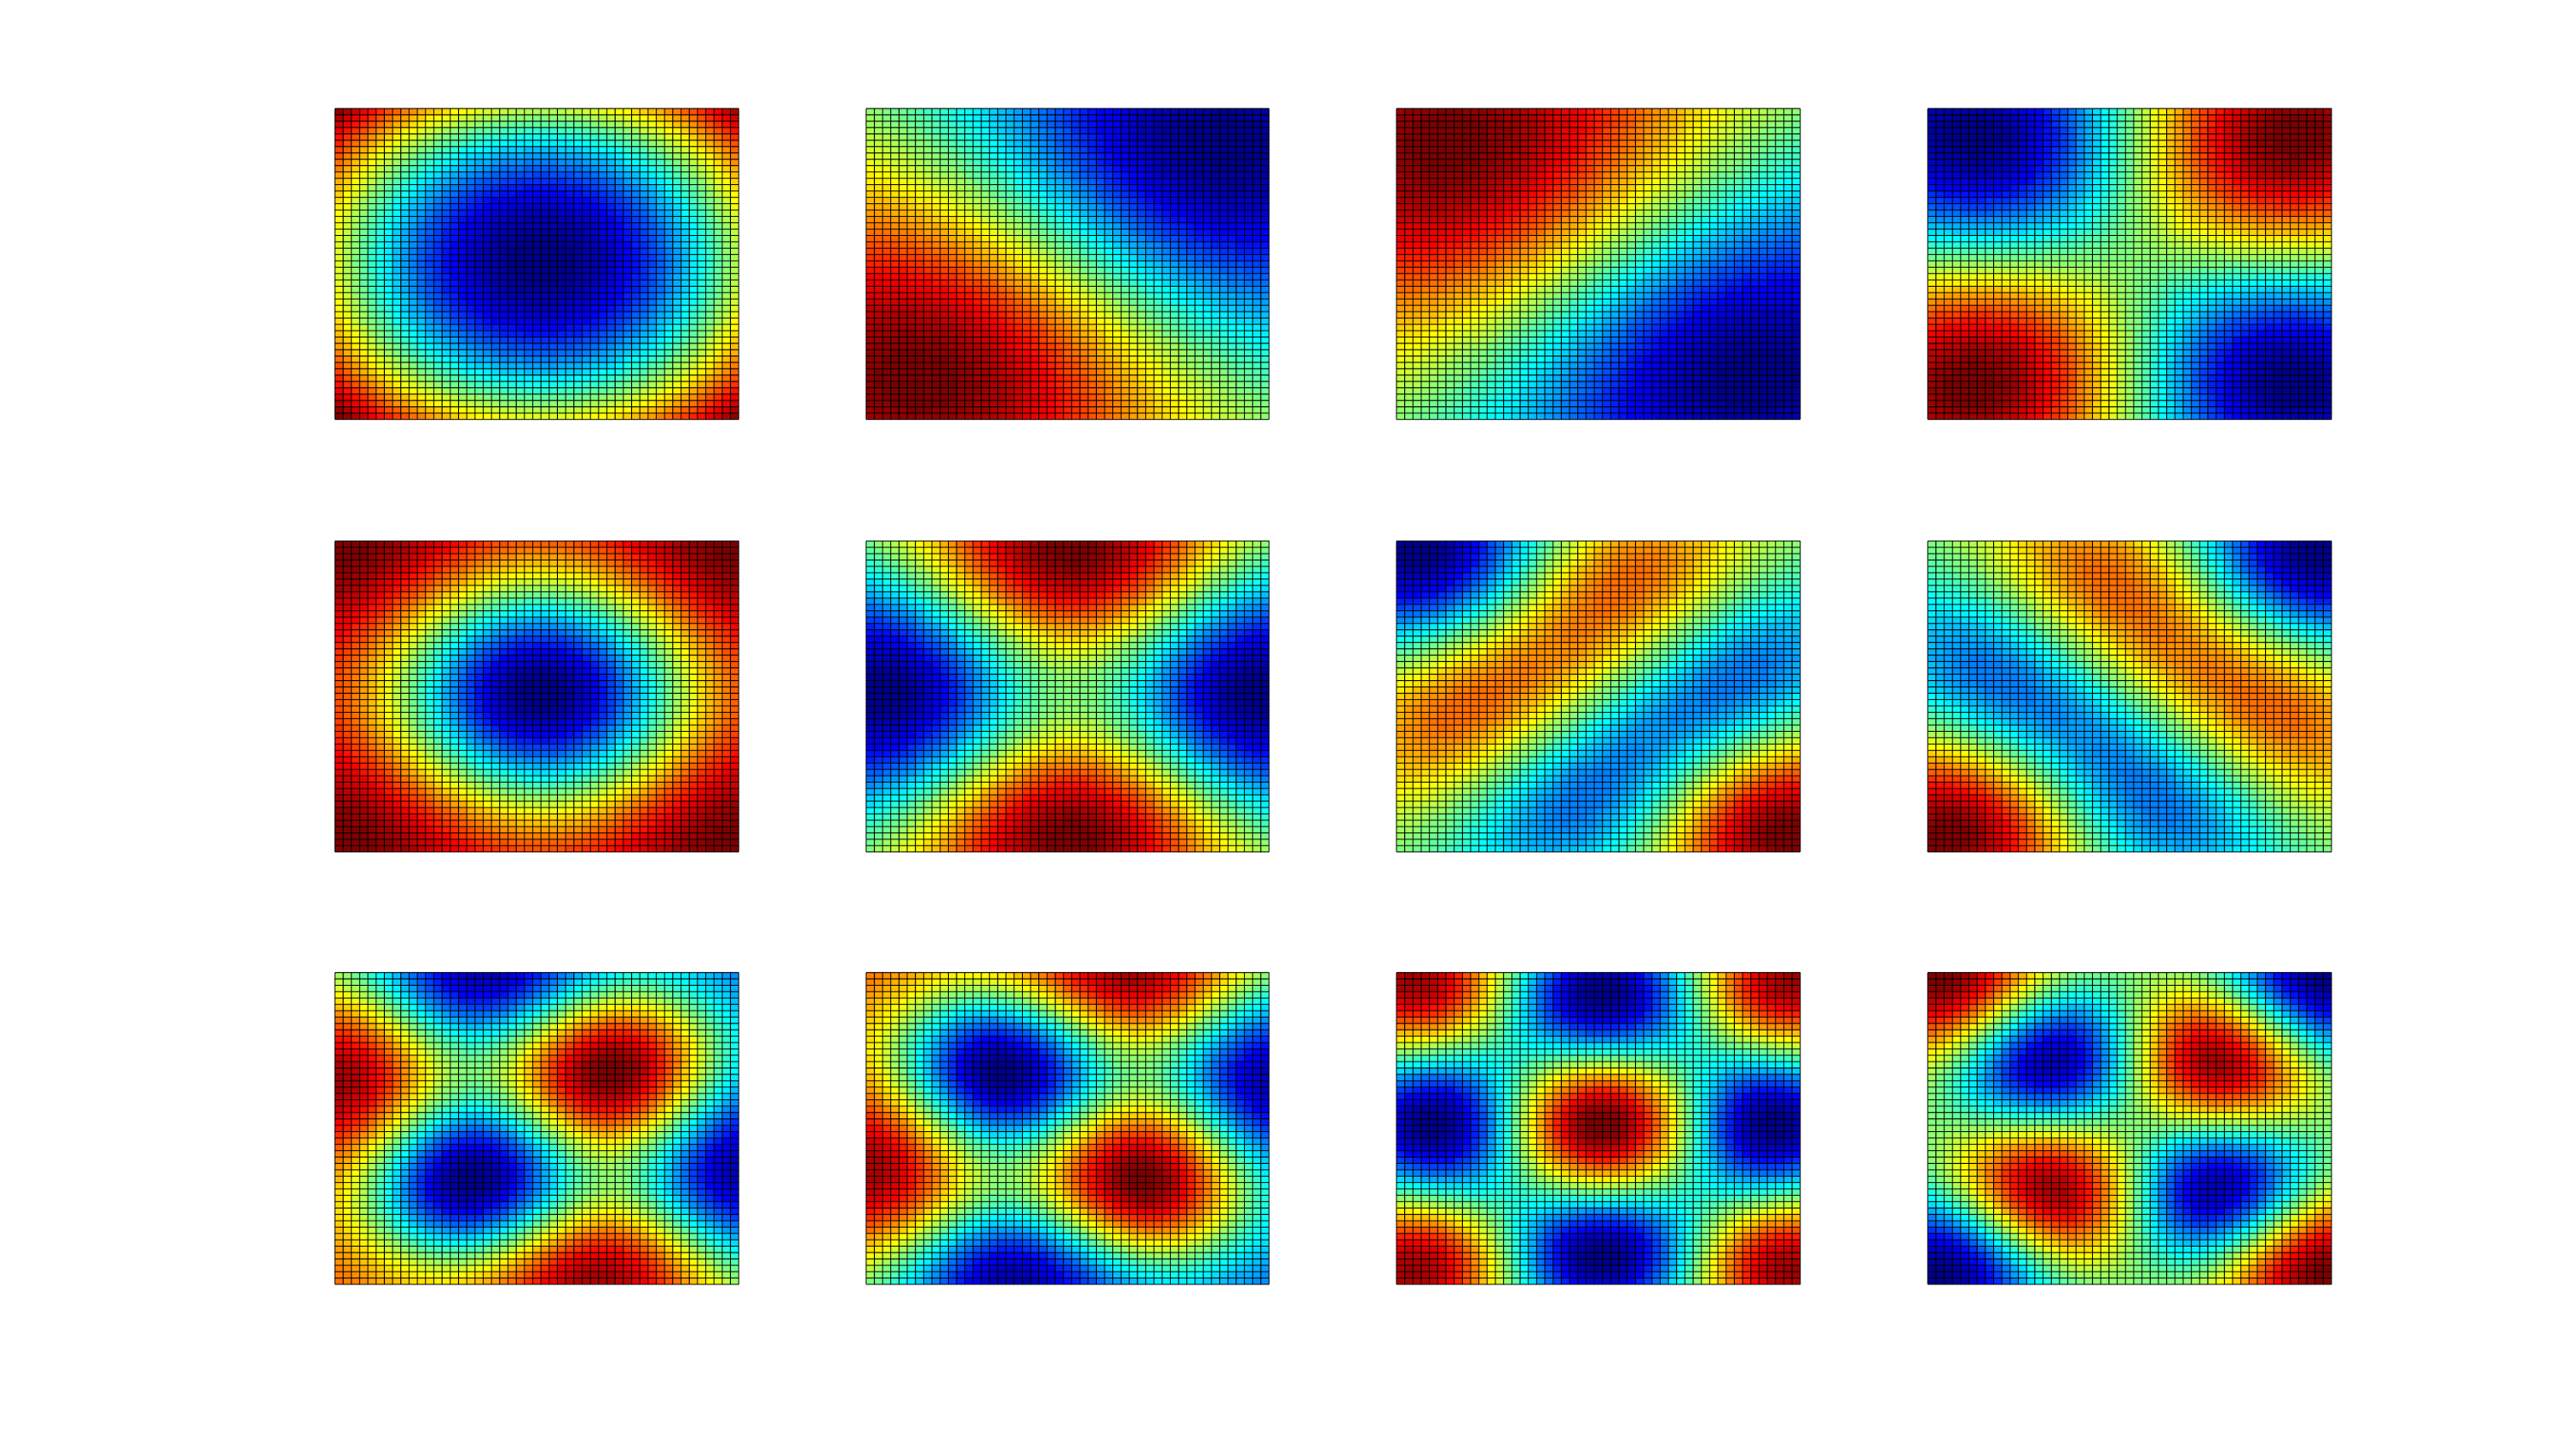
\includegraphics[width=\textwidth]{Images/recBasis.png}
\end{center}
\end{frame}


% crazy cov
\begin{frame}
\frametitle{(M2) Climate Variability Covariance $\C$}
\framesubtitle{Modified eigenfunction covariance $\C = V_{exp} \tilde \Lambda V_{exp}^{-1}$}
\begin{columns}
\begin{column}{0.5\textwidth}
    \begin{center}
     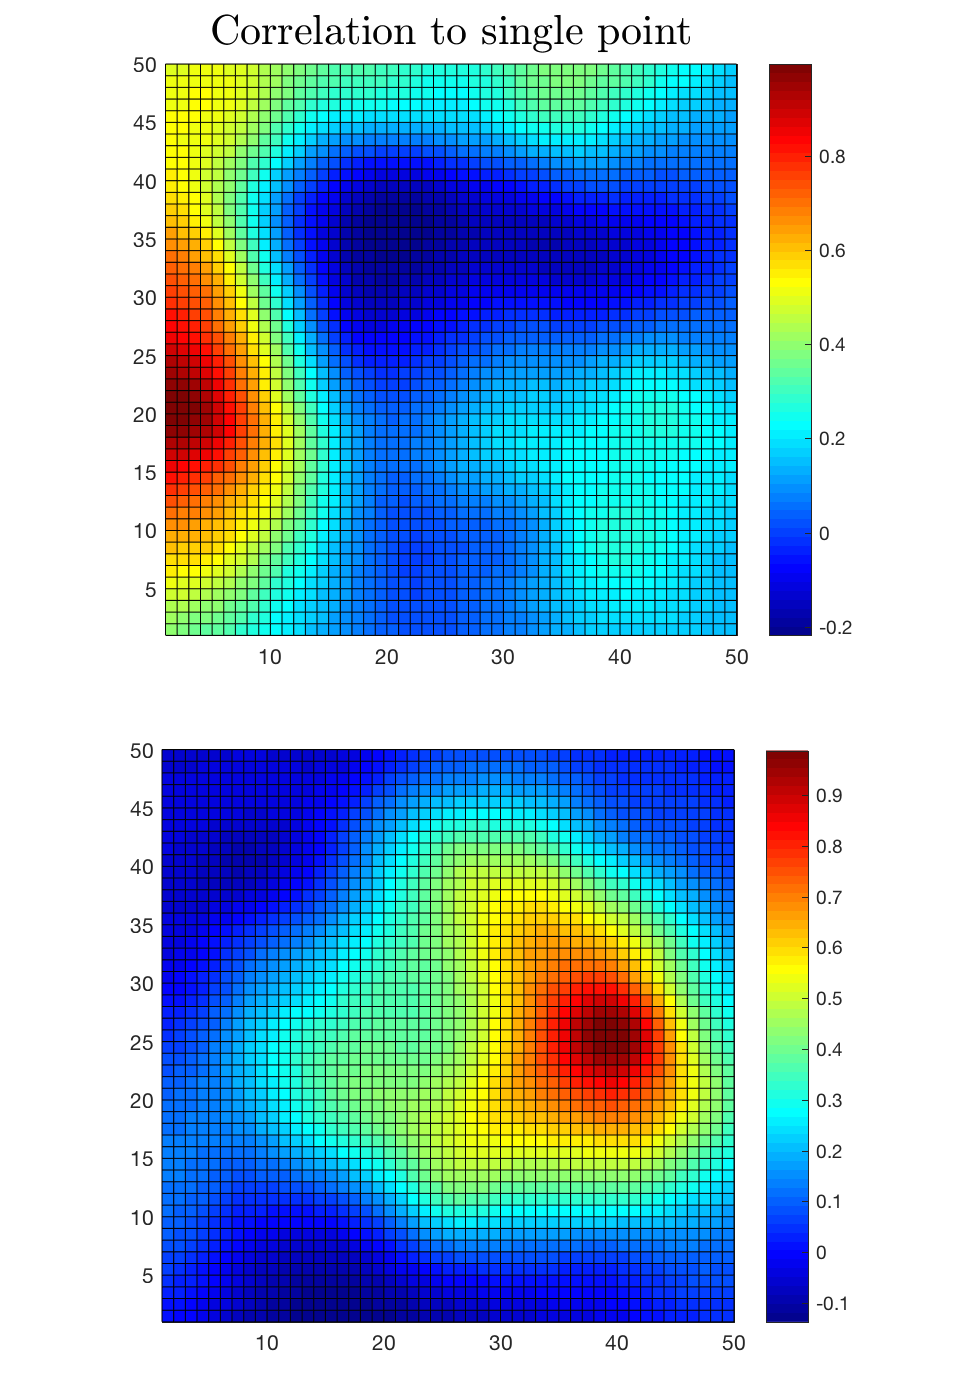
\includegraphics[width=0.90\textwidth]{Images/modCorrelation.png} 
     \end{center}
\end{column}
\begin{column}{0.5\textwidth}
    \begin{center}
     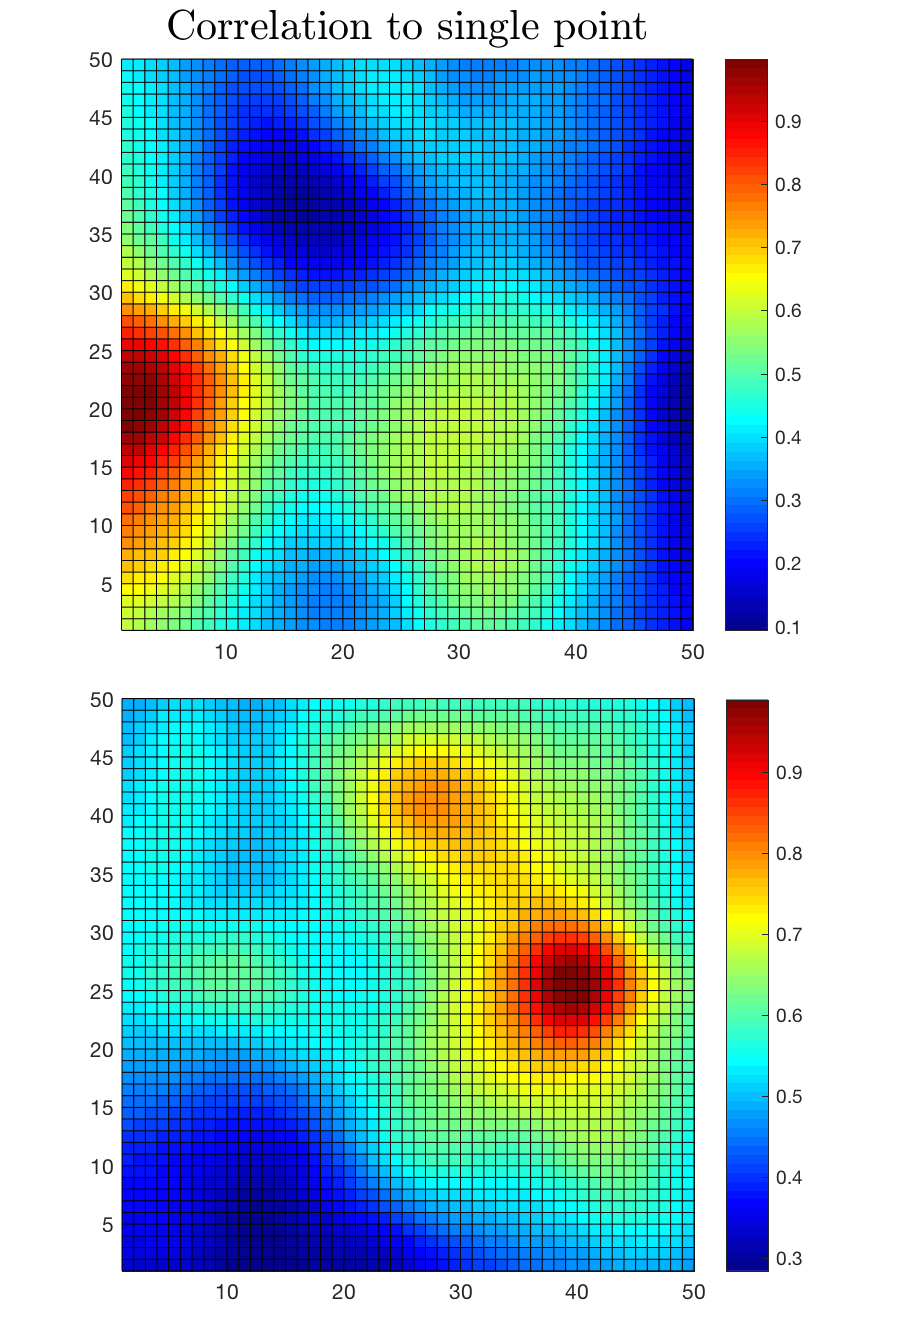
\includegraphics[width=0.88\textwidth]{Images/modCorrelation2.png} 
     \end{center}
\end{column}
\end{columns}
\end{frame}



% Simulation Outline
\begin{frame}
\frametitle{Simulation Procedure}

\begin{block}{}
\vspace*{-\baselineskip}\setlength\belowdisplayshortskip{0pt}
\begin{alignat*}{3}
\*y_{obs} &= \*y_{rel} + \*\varepsilon_y  \qquad \quad &\*\varepsilon_y &\sim \mathcal N(0,\W)\\
\*y_{rel} &= \*X^* \*\beta + \*u_y \nonumber  \qquad  &\*u_y &\sim \mathcal N(0,\alpha^{-1}\,\C) \\
\overline{\*X} &= \*X^* + \*L^{-1/2} \*U \qquad    &\*u_m &\stackrel{\text{ind}}{\sim} \mathcal N(0,\gamma_m^{-1} \, \C)  \:
\end{alignat*}
\end{block}

For a simulation of fixed dimensionality:
\begin{itemize}
\item[\light{1)}] \light{Set/Simulate fixed objects $\theta = \{ \beta, \alpha, \*\gamma , \C, \W \}$ and $\*X^*$
\begin{itemize}
\item \light{$\*X^*$, $\C$, and $\W$ according to simulation modules}
\end{itemize}
}
\item[2a)] Simulate the observed forcing response ensembles $\*x_m$ 
\[
\*x^{(\ell)}_m \iid \mathcal N ( \*x_m^*, \C)
\]
\item[2b)] Simulate the realized climate response $\* y_{rel}$
\[
\*y_{rel} \sim \mathcal N ( \*X^* \* \beta, \C)
\]
\item[\light{3)}] \light{Simulate the observed climate response ensemble $\*Y_{obs}$}
\light{\[
\*y_{obs}^{(\ell)} \iid \mathcal N ( y_{rel}, \W)
\]}
\end{itemize}
\end{frame}


% X response progression

\begin{frame}
\frametitle{2a) Simulate the Observed Forcing Responses}
\framesubtitle{$\*x^{(\ell)}_m \iid \mathcal N ( \*x_m^*, \gamma_m^{-1} \C)$}
\begin{center}
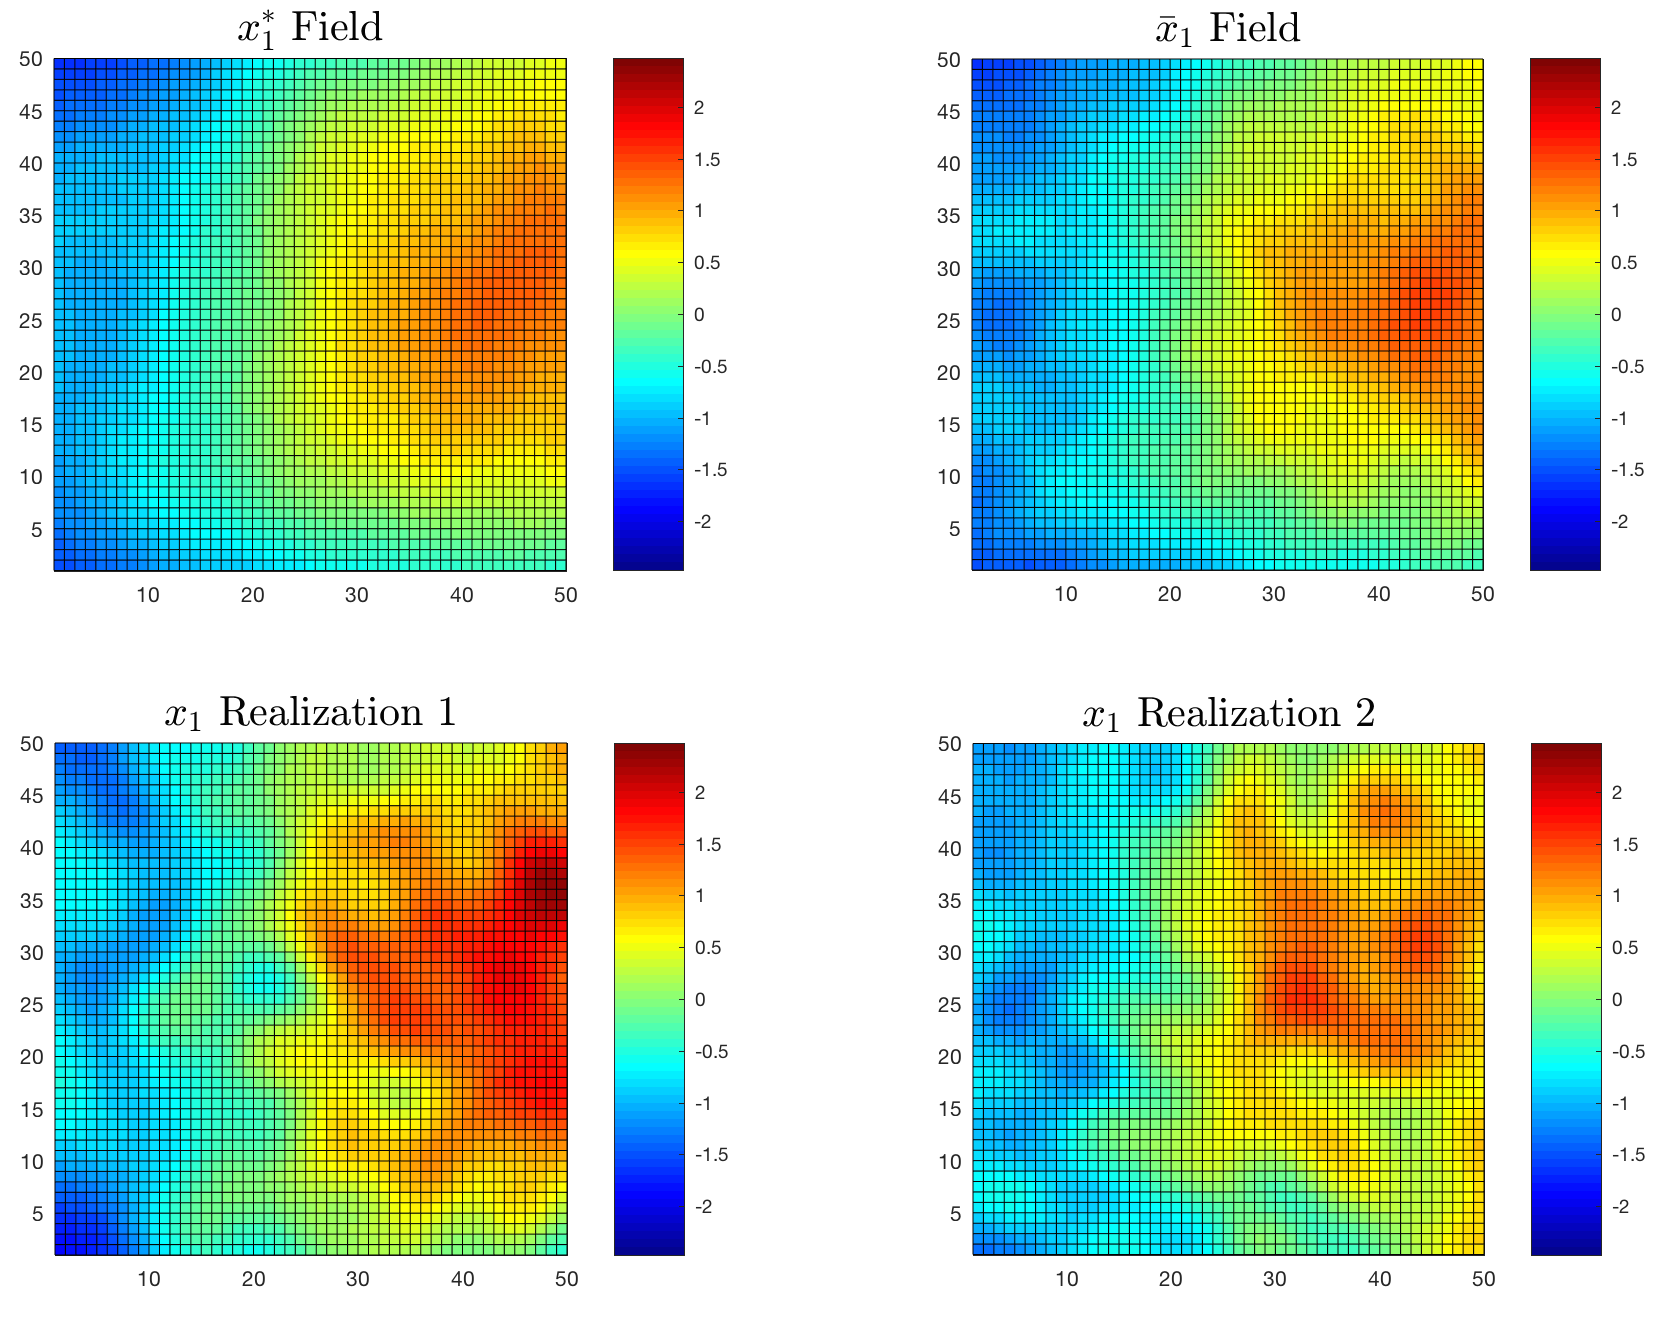
\includegraphics[width=0.75\textwidth]{Images/xGeneration.png}
\end{center}
\end{frame}


% Y_rel progression

\begin{frame}
\frametitle{2b) Simulate the Realized Climate Response}
\framesubtitle{$\*y_{rel} \sim \mathcal N ( \*X^* \* \beta, \alpha^{-1} \C)$}
\begin{center}
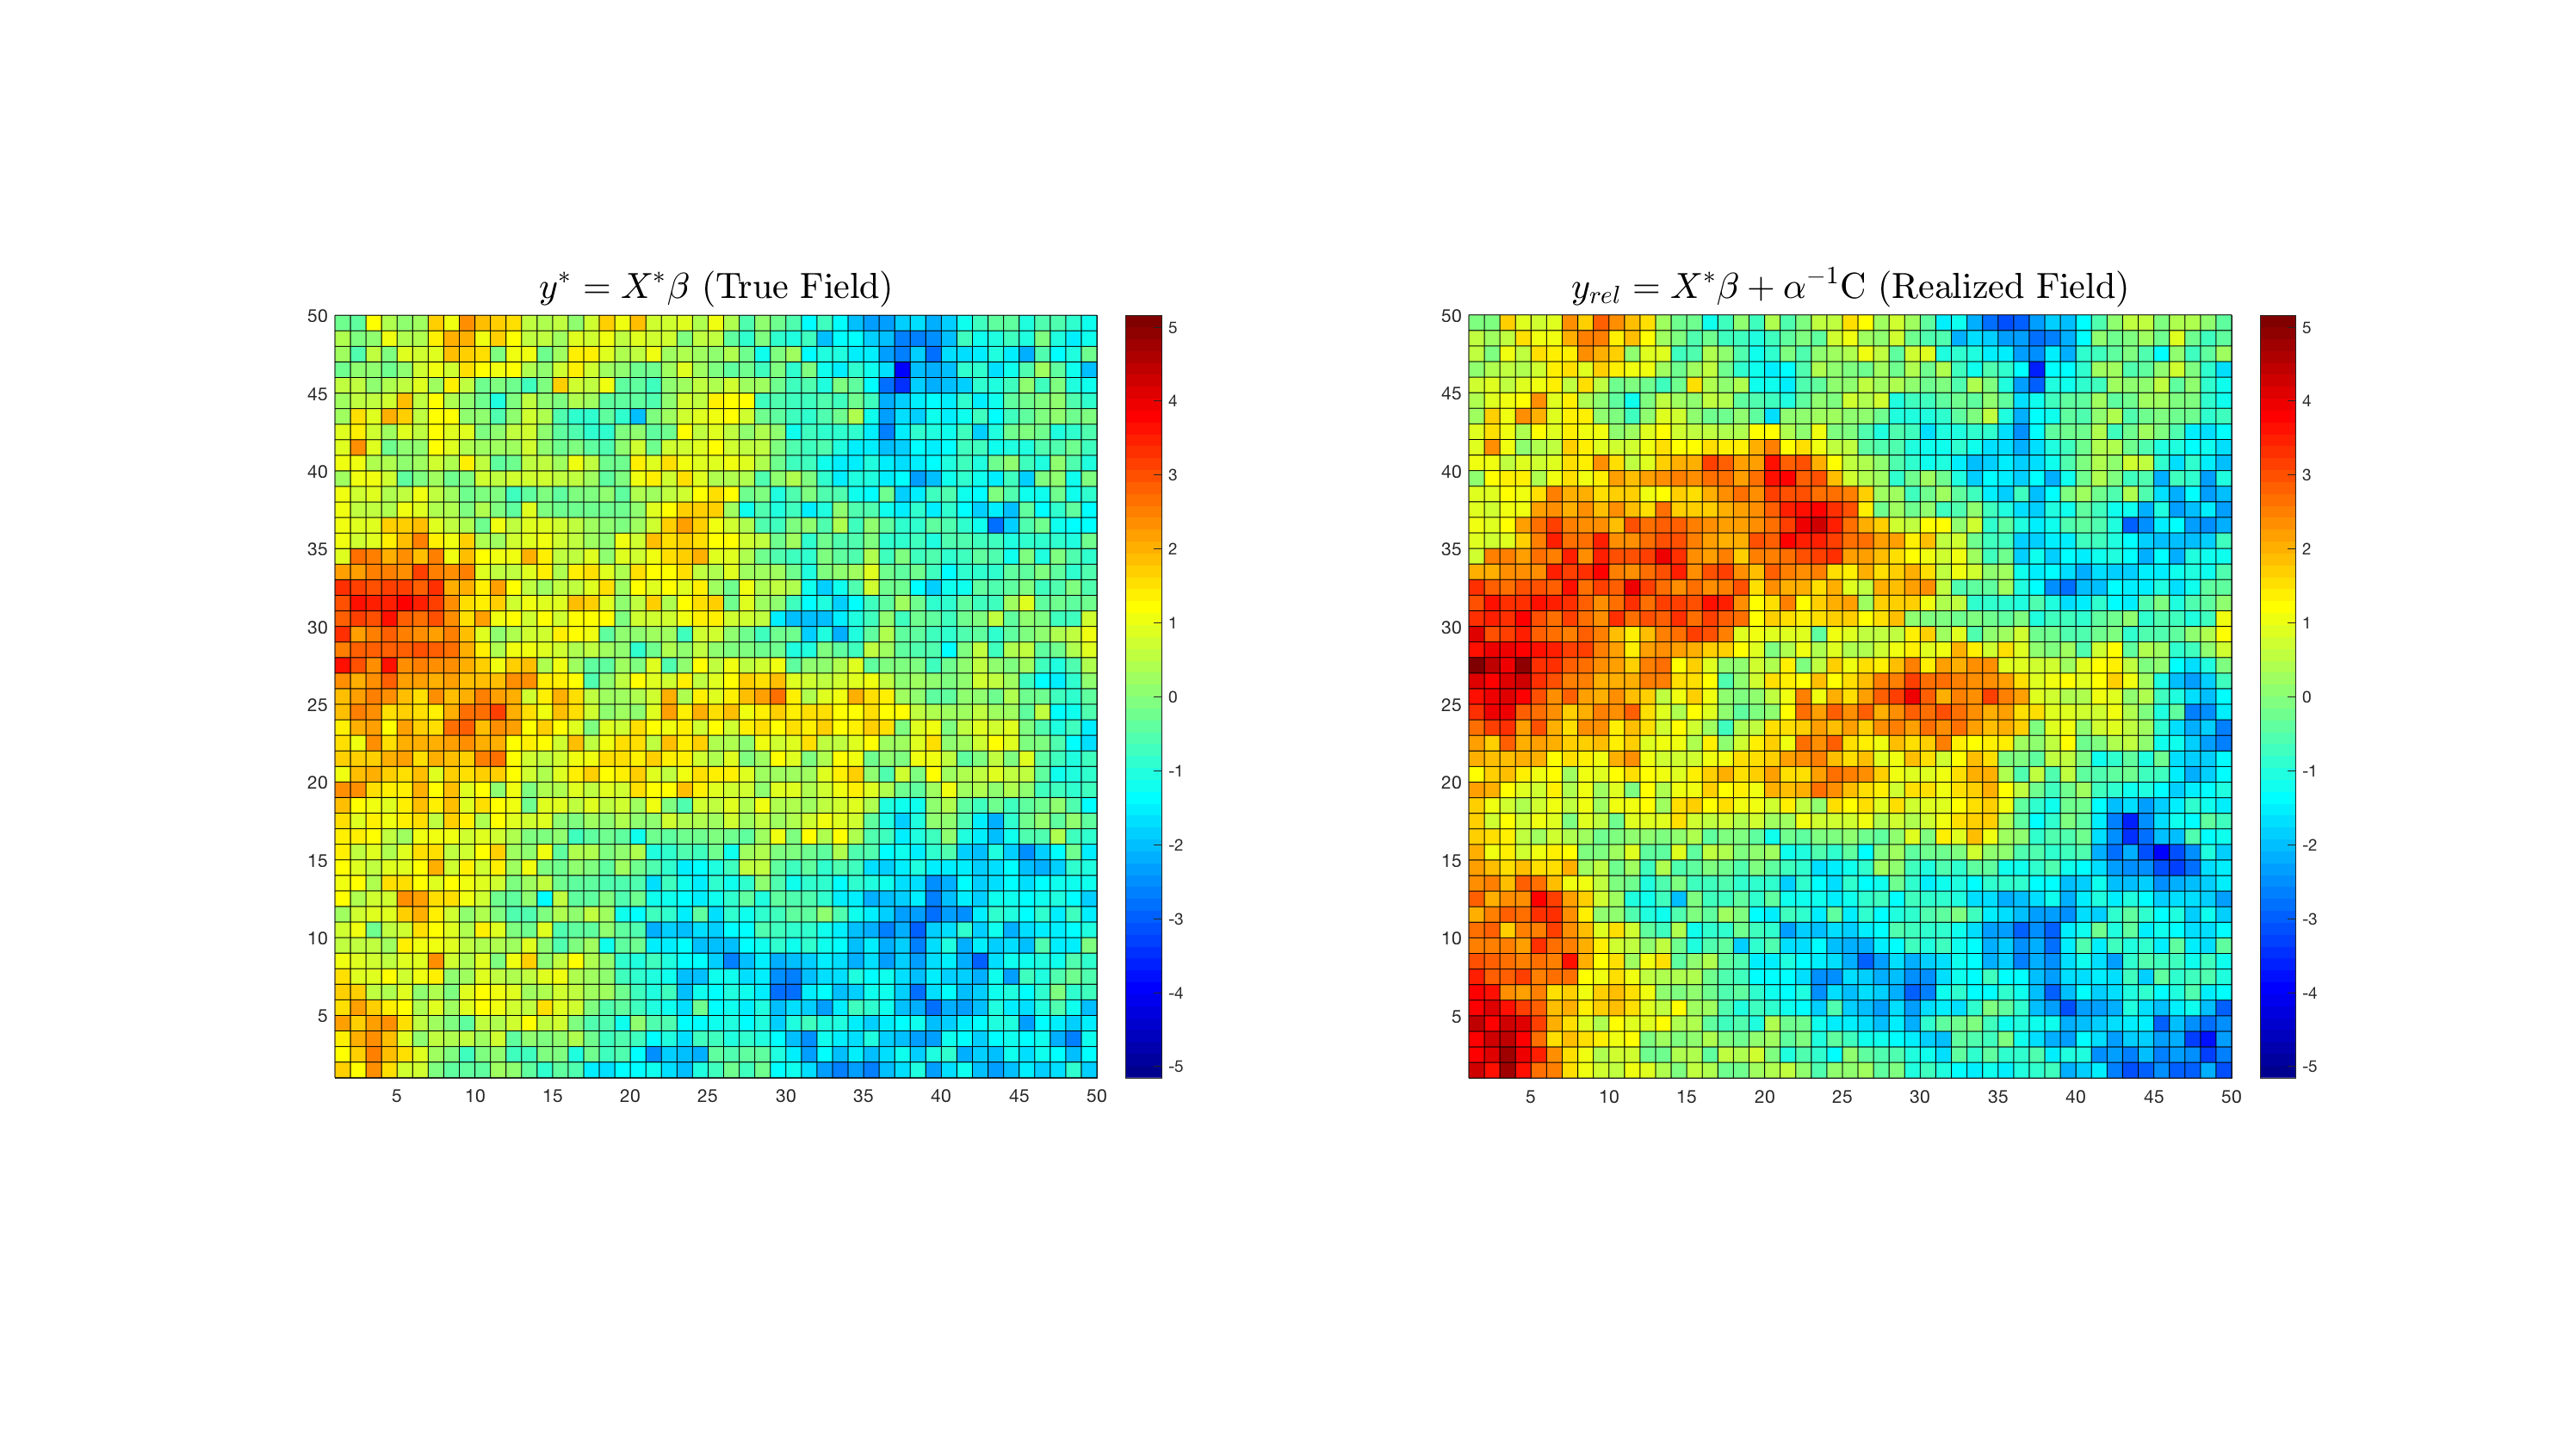
\includegraphics[width=\textwidth]{Images/yprogression.png}
\end{center}
\end{frame}

\begin{frame}
\frametitle{Simulation Procedure}

\begin{block}{}
\vspace*{-\baselineskip}\setlength\belowdisplayshortskip{0pt}
\begin{alignat*}{3}
\*y_{obs} &= \*y_{rel} + \*\varepsilon_y  \qquad \quad &\*\varepsilon_y &\sim \mathcal N(0,\W)\\
\*y_{rel} &= \*X^* \*\beta + \*u_y \nonumber  \qquad  &\*u_y &\sim \mathcal N(0,\alpha^{-1}\,\C) \\
\overline{\*X} &= \*X^* + \*L^{-1/2} \*U \qquad    &\*u_m &\stackrel{\text{ind}}{\sim} \mathcal N(0,\gamma_m^{-1} \, \C)  \:
\end{alignat*}
\end{block}

For a simulation of fixed dimensionality:
\begin{itemize}
\item[\light{1)}] \light{Set/Simulate fixed objects $\theta = \{ \beta, \alpha, \*\gamma , \C, \W \}$ and $\*X^*$
\begin{itemize}
\item \light{$\*X^*$, $\C$, and $\W$ according to simulation modules}
\end{itemize}
}
\item[\light{2a)}] \light{Simulate the observed forcing response ensembles $\*x_m$ 
\[
\*x^{(\ell)}_m \iid \mathcal N ( \*x_m^*, \C)
\]
\item[\light{2b)}] Simulate the realized climate response $\* y_{rel}$
\[
\*y_{rel} \sim \mathcal N ( \*X^* \* \beta, \C)
\]
}
\item[3)] Simulate the observed climate response ensemble $\*Y_{obs}$
\[
\*y_{obs}^{(\ell)} \iid \mathcal N ( y_{rel}, \W)
\]
\end{itemize}
\end{frame}

% Y_obs progression

\begin{frame}
\frametitle{3) Simulate the observed climate response}
\framesubtitle{$\*y_{obs}^{(\ell)} \iid \mathcal N ( y_{rel}, \W)$}


\begin{columns}
\begin{column}{0.5\textwidth}
    \begin{center}
     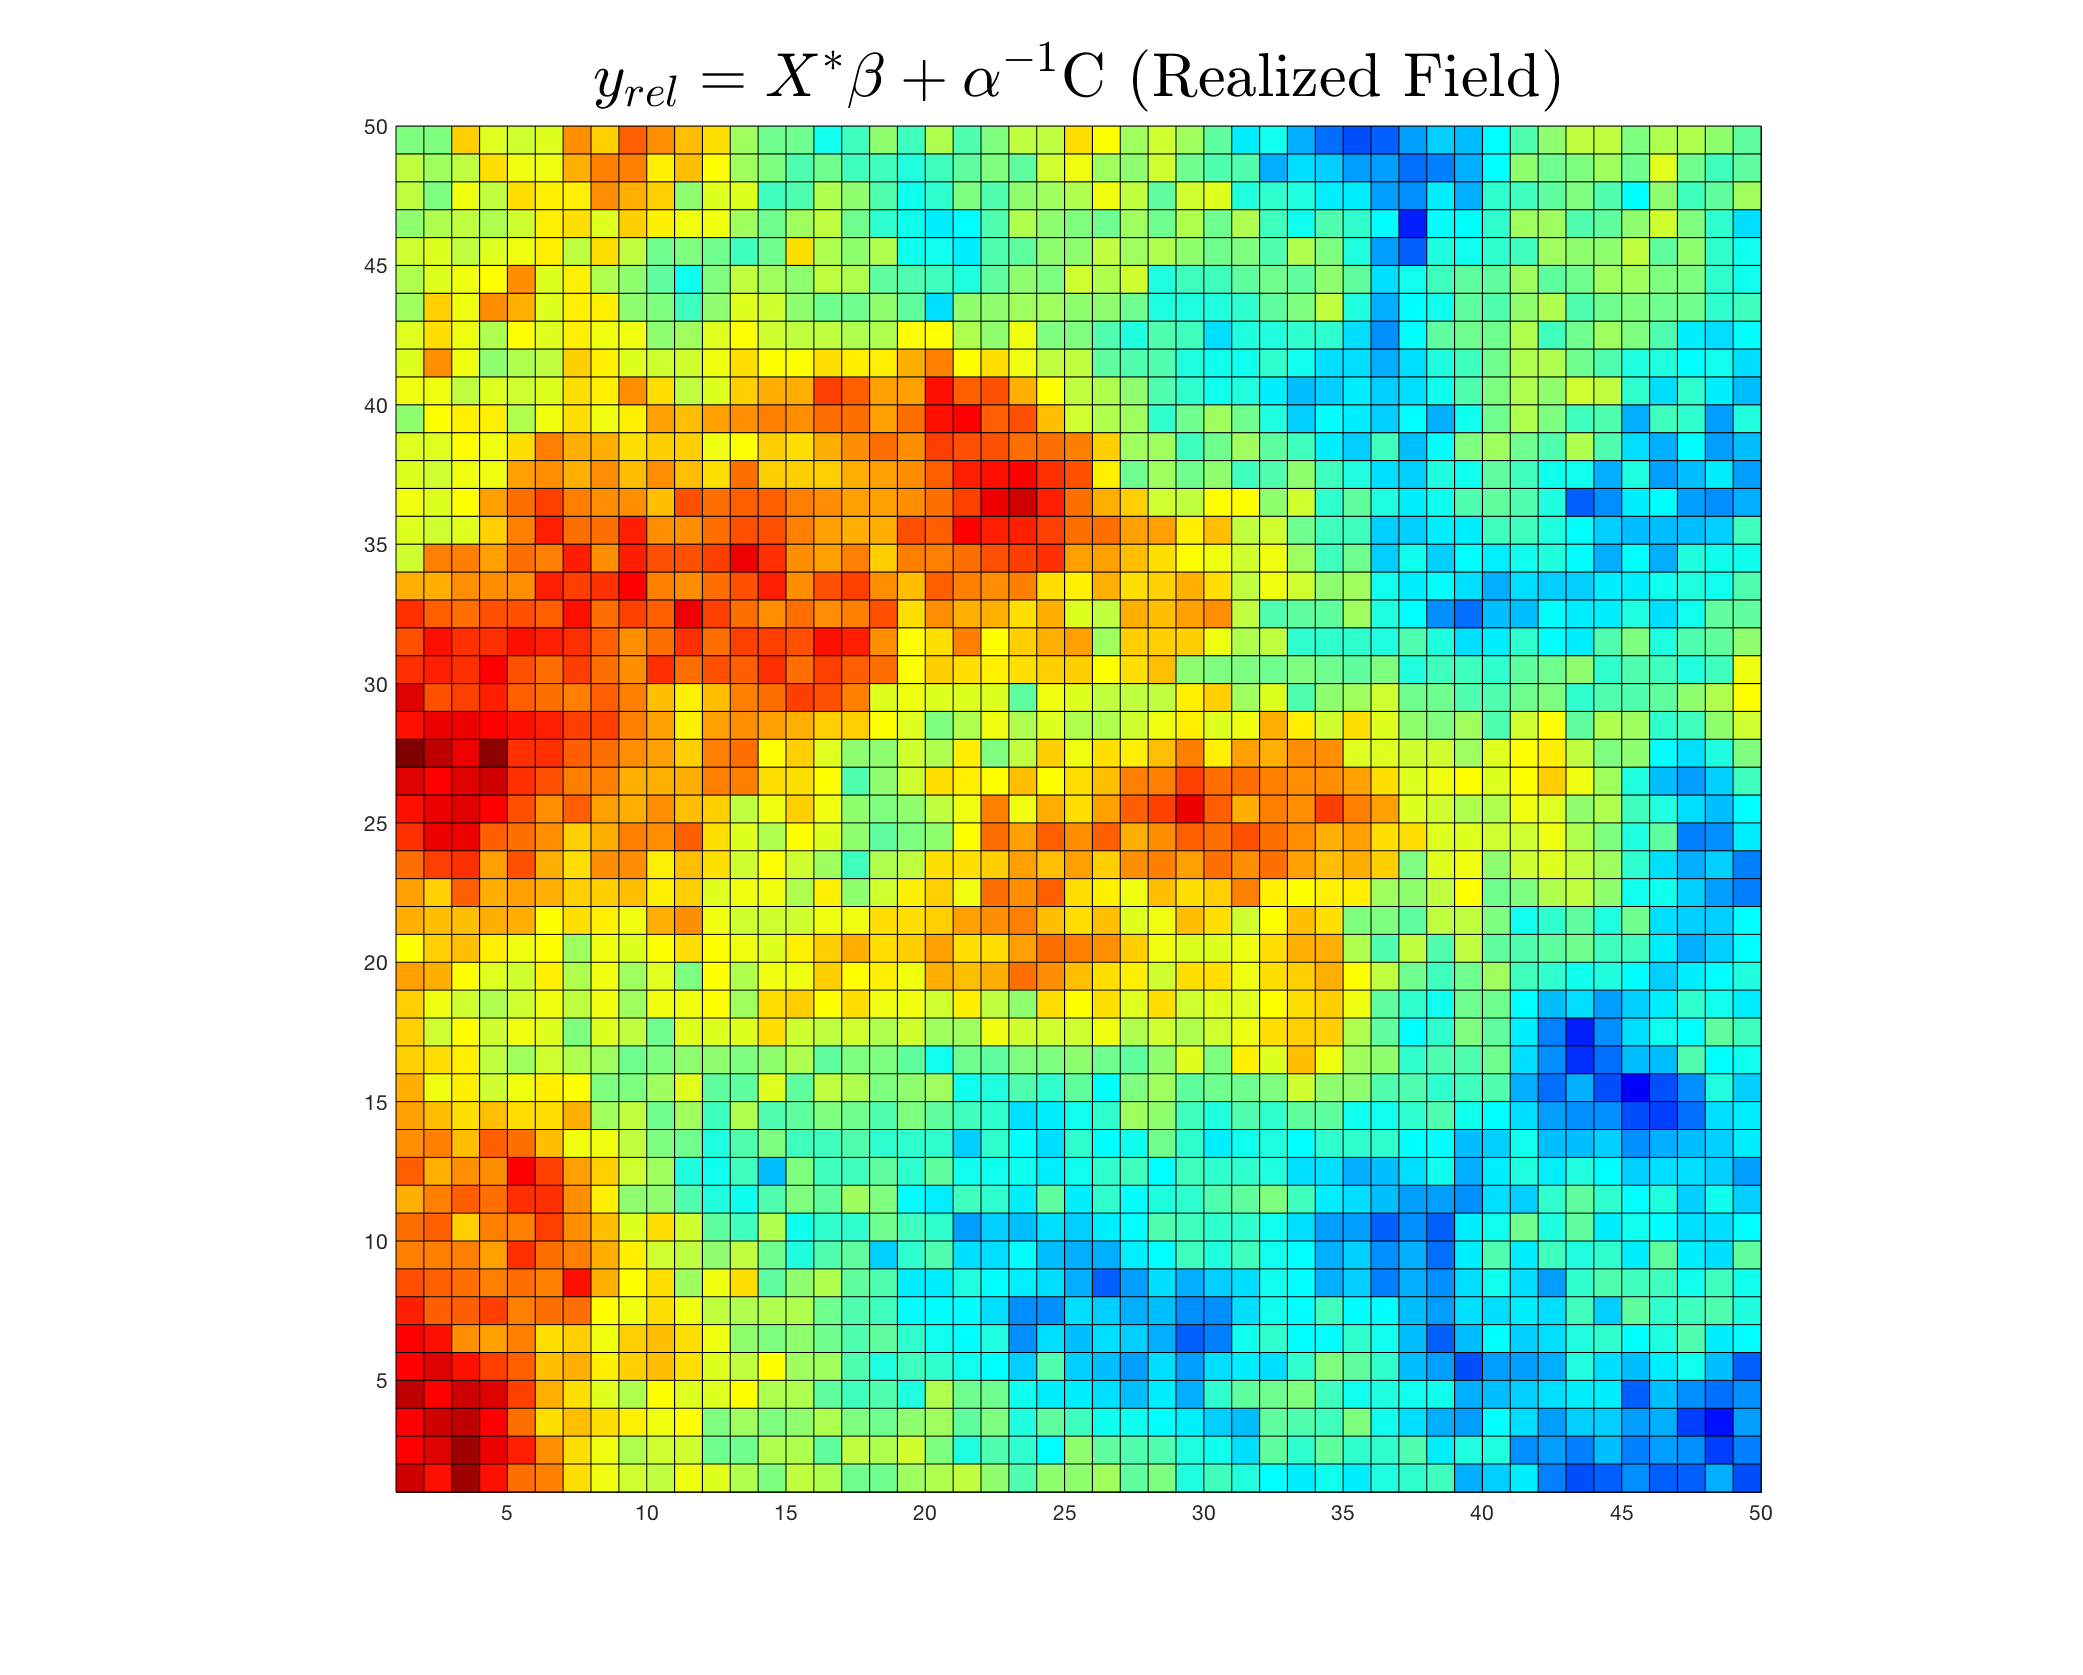
\includegraphics[width=0.95\textwidth]{Images/yrealized.png} 
     \end{center}
\end{column}
\begin{column}{0.5\textwidth}
    \begin{center}
     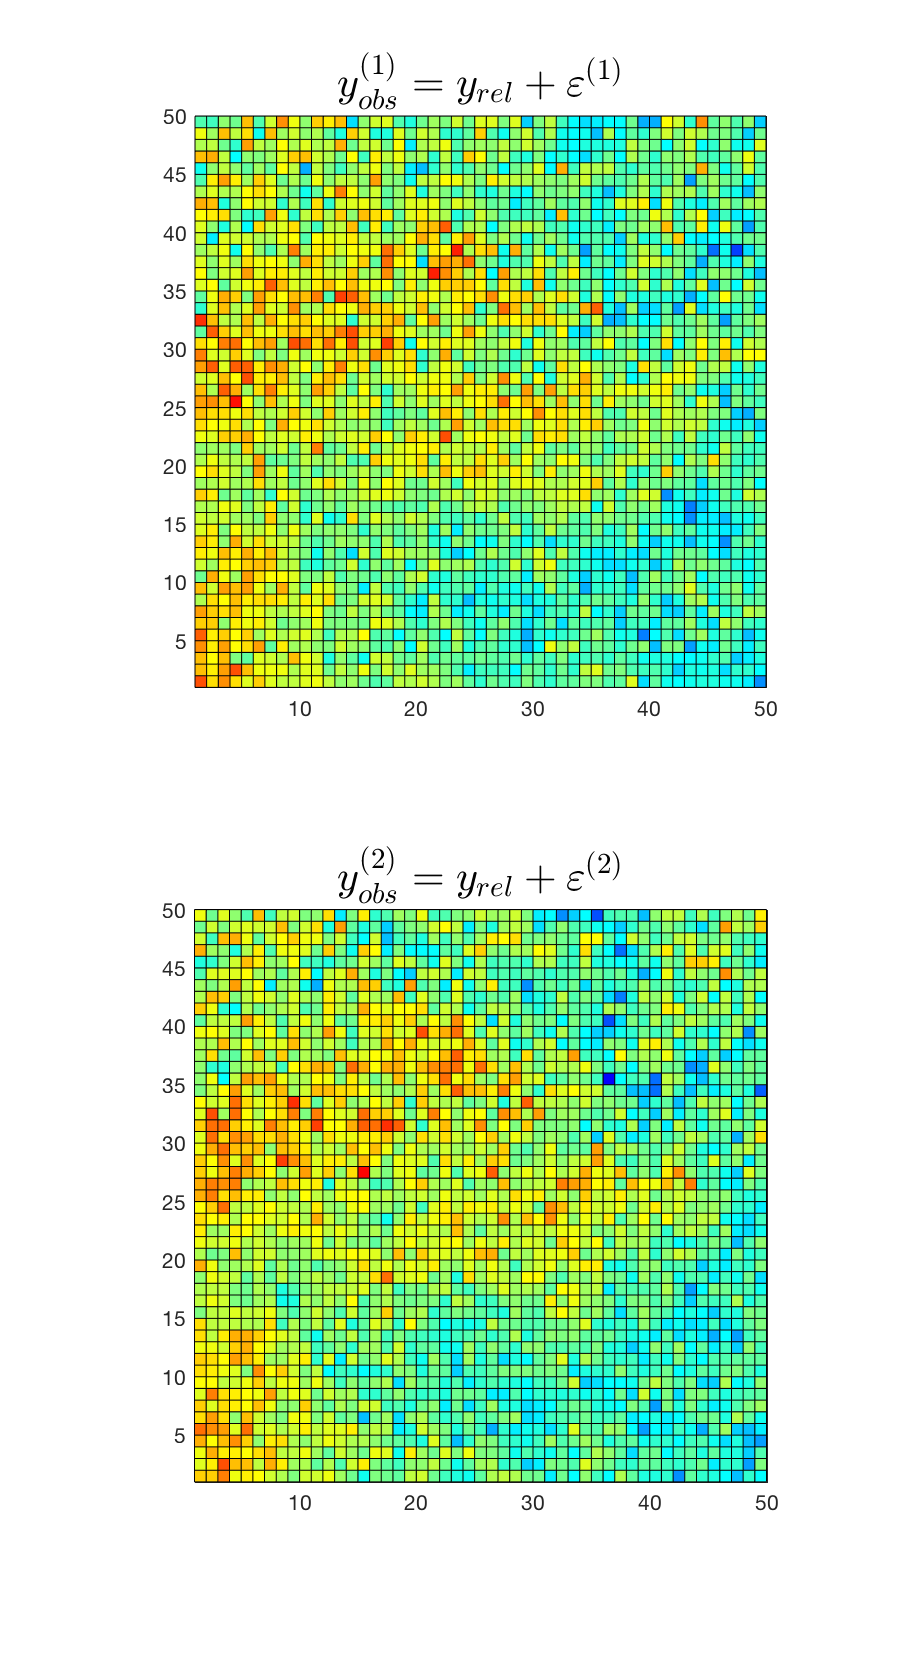
\includegraphics[width=0.75\textwidth]{Images/yobservation.png} 
     \end{center}
\end{column}
\end{columns}

\end{frame}

% Discussion list
\begin{frame}
\frametitle{Discussion and Next Steps}
\begin{itemize}
\item \structure{Current Testbed}
\begin{itemize}
\item Flexible, fast generation of EIV Detection and Attribution data
\item Non-isotropic climate variability
\end{itemize}

\item \structure{First Applications}
\begin{itemize}
\item Used in testing new method from Smith, Hammerling and Johnson
\end{itemize}

\item \alert{Next Steps}
\begin{itemize}
\item Fit forcing responses and sources of variability to real applications
\item Compare traditional OLS and TLS methods as a function of testbed parameters
\item Evaluate models from \cite{hannart16} and \cite{khs17}
\end{itemize}
\item Thank you/Input/Requests
\end{itemize}

\end{frame}

\begin{frame}
\frametitle{References}
\bibliographystyle{apalike}

\bibliography{idagTalk}
\end{frame}

\end{document}